\chapter{Fock Matrix prediction: A first trial}
\label{chap:fock_matrix_predictions}

SCF methods by nature initially need a density matrix to start off their iterative calculations. Independent of the way the initial guess is chosen the computational effort of this step should be negligible compared to the actual SCF iterations. 
\TODO{Add more details about the Fock matrix prediction - Reasoning for the choice.}

As explained in \autoref{sec:background} (\TODO{Background SCF}) the density matrix $P$ is calculated from the coefficient matrix $C$ which is obtained from the eigenvalue problem of the Fock matrix $F$:
\begin{equation}
    F(P)\,C = SC\varepsilon \rightarrow P = 2\,\sum_{i}^{n_{occ}} C_{\mu i}\,C^*_{\nu i}\,,%2CC^T
\end{equation}
Effectively, one performs part of the SCF cycle here to obtain the density matrix, which ideally should be close to the final density matrix. This step takes $\bigO{N^3}$ time, which is assymtotically faster than the $\bigO{N^4}$ time of the SCF cycle. 


\noindent
\begin{figure}[H]
    \centering
    \begin{tikzpicture}[scale=1, every node/.style={transform shape}]

        % Skalierungsfaktor für drei Bilder + Zwischenraum
        \def\imgwidth{0.30\linewidth}

        % Erstes Bild mit Titel
        \node[anchor=south west, inner sep=0] (img1) at (0,0)
            {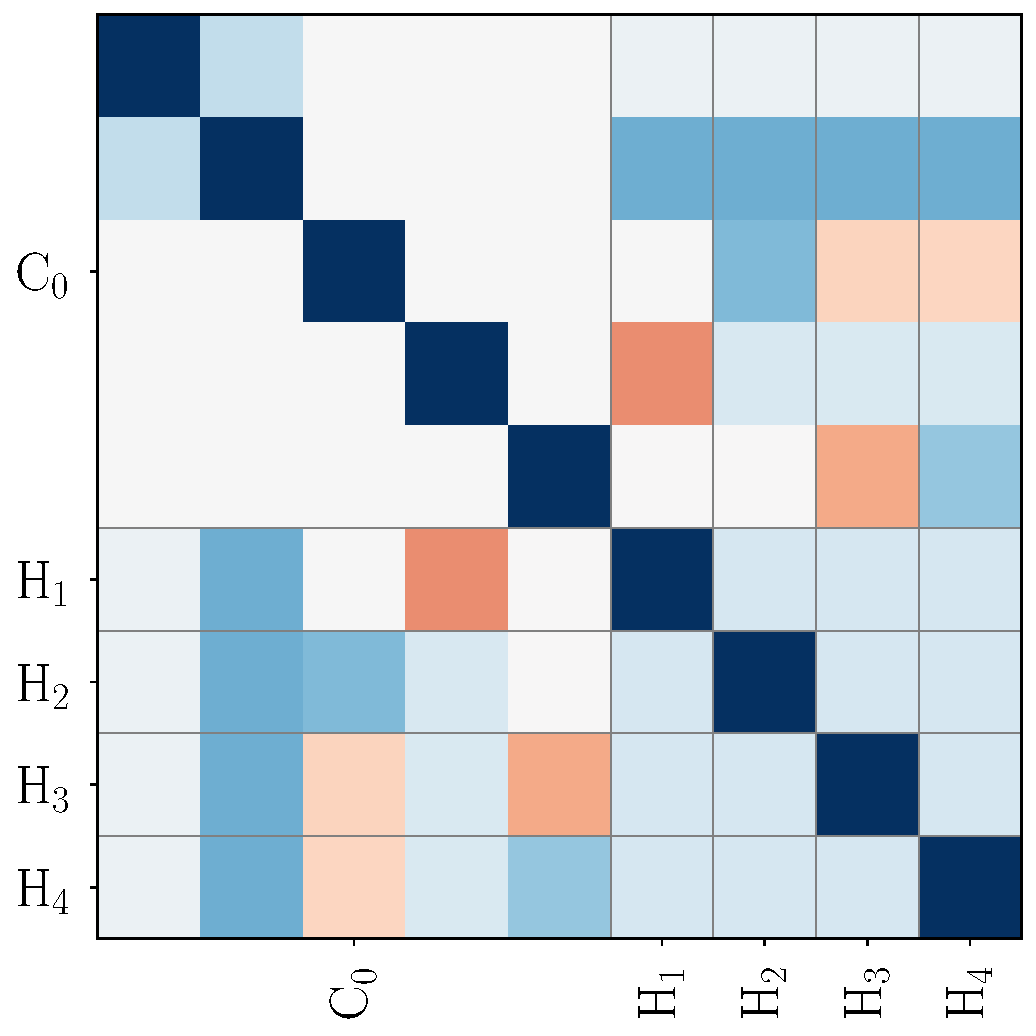
\includegraphics[width=\imgwidth]{../fig/c5h4n2o2/overlap_dsgdb9nsd_000001.pdf}};
        \node[above=2pt of img1.north, anchor=south, font=\small, xshift=10pt] {Overlap};

        % Zweites Bild mit Titel
        \node[anchor=south west, inner sep=0] (img2) at (5.1,0)
            {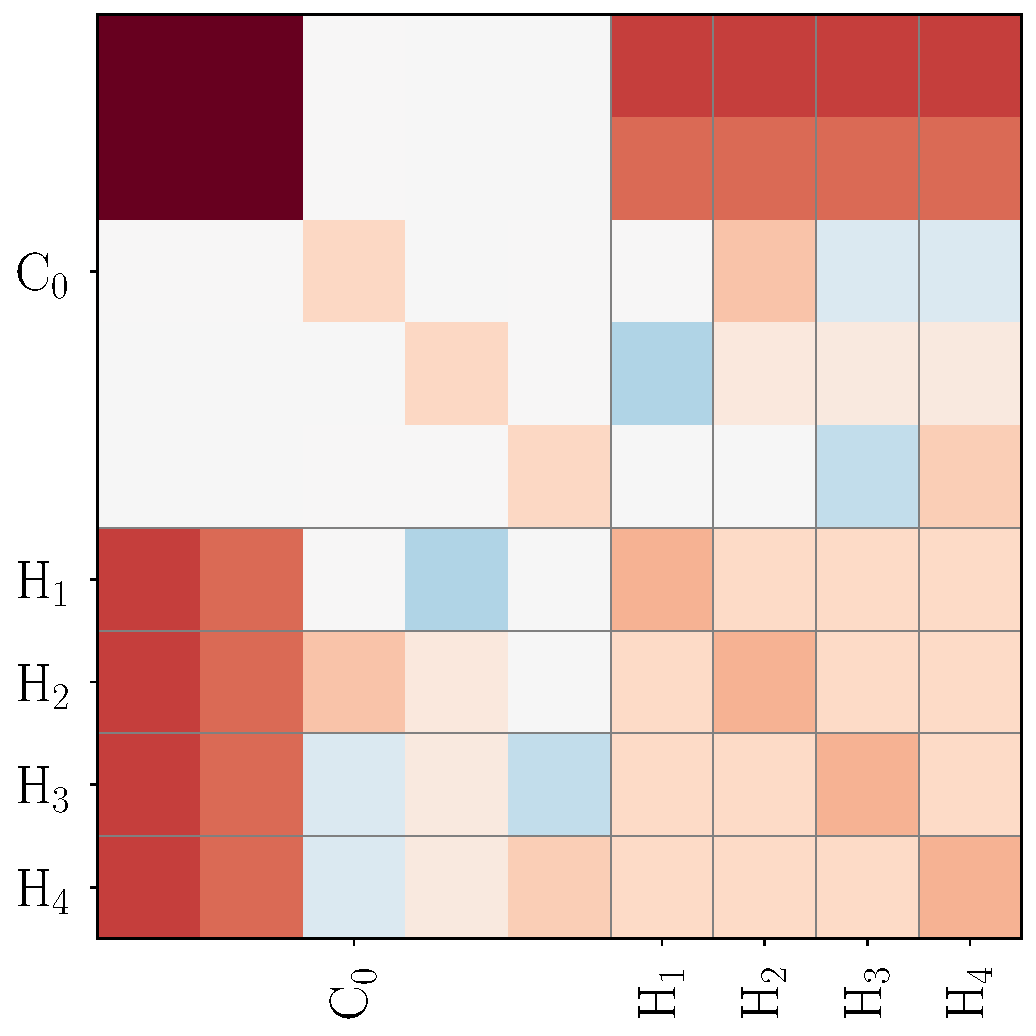
\includegraphics[width=\imgwidth]{../fig/c5h4n2o2/fock_dsgdb9nsd_000001.pdf}};
        \node[above=2pt of img2.north, anchor=south, font=\small, xshift=10pt] {Fock};

        % Drittes Bild mit Titel
        \node[anchor=south west, inner sep=0] (img3) at (10.2,0)
            {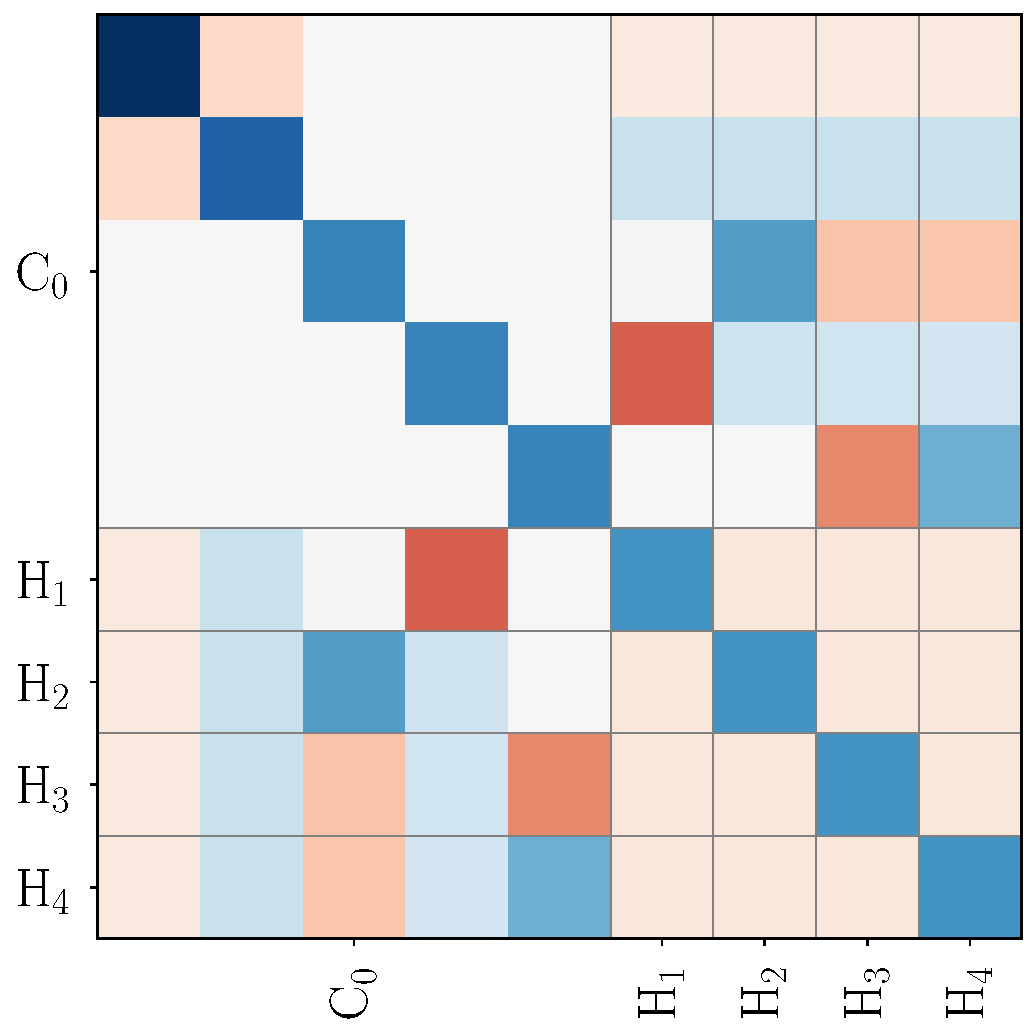
\includegraphics[width=\imgwidth]{../fig/c5h4n2o2/density_dsgdb9nsd_000001.pdf}};
        \node[above=2pt of img3.north, anchor=south, font=\small, xshift=10pt] {Density};
        
        % Pfeil 1: ML model
        \draw[->, thick] (4.7,2.4) -- node[above, align=center, font=\tiny]{ML\\model} (5.2,2.4);

        \draw[->, thick] (9.8,2.4) -- node[above, font=\tiny, yshift=1pt]{$P{=}2CC^{\mathrm{T}}$} (10.3,2.4);
    \end{tikzpicture}
    \caption[Schematic overview data flow]{Schematic overview of the data flow (using \ch{CH4}): overlap matrix to Fock matrix via ML model prediction, and construction of the density matrix from the Fock matrix.}
    \label{fig:method_data_flow}
\end{figure}

The schematic workflow of generating a density matrix from the overlap matrix is shown in \autoref{fig:method_data_flow}. While the overlap and density might look very similar and one might think that predicting the density matrix directly from the overlap matrix would be easier. However, learning the Fock matrix tends to involve fewer strict physical constraints. A Fock matrix primarily needs to be Hermitian, while a density matrix must be strictly positive semidefinite by construction, as well as normalized to the correct number of electrons. That makes direct density matrix learning more challenging, whereas learning the Fock matrix and then obtaining the density through the diagonalization could yield better results. \TODO{Reference?}

\section{\ch{C5H4N2O2}-subset: A first trial}
\label{sec:qm9_c5h4n2o2}

As a proof of concept we will use 508 constitutional isomers\footnote{From the 509 constitutional isomers of \ch{C5H4N2O2} 508 converged using the STO-3G basis and the B3LYP functional.} of \ch{C5H4N2O2} from the QM9 dataset. 
Single point RKS simulations in \textsc{PySCF} \parencite{ref:pyscf} were performed for these molecules using the B3LYP\footnote{B3LYPG was used to be consitant with the Gaussian} functional and the STO-3G basis. The resulting converged density-, fock-, and overlap-matrices were saved for future training purposes. For our very minimal basis these matrices are of size $49 \times 49$ as can be seen for a converged density in \autoref{fig:density_dsgdb9nsd_022700}. 
Due to the symmetry of the matrices we can discard nearly half of the elements and are left with 1225 features to learn. A rule of thumb for training classical statistical models is to have at least 10 samples per feature. \parencite{ref:rule_of_10} The given dataset of 508 samples is therefore far off from this rule if we discard multiplicity in atoms in the samples. As a first step we shall limit our efforts to single models predicting the system based on the full overlap matrix. Nevertheless, the row / column order of our atoms in the overlap matrix has to be consistent for all the samples in the dataset (as seen in \autoref{fig:density_dsgdb9nsd_022700}). This will simply be done by sorting the atoms in the overlap matrix according to their atomic number. Now we are ready to start off our endeavour with a Ridge regression model as a first trial. 

\begin{figure}[H]
    \centering
    \includegraphics[width=\textwidth]{../fig/c5h4n2o2/density\_dsgdb9nsd\_022700.pdf}
    \caption[Density matrix of dsgdb9nsd\_022700 in the STO-3G basis with theory level B3LYP]{Converged density of dsgdb9nsd\_022700 in the STO-3G basis with theory level B3LYP. The density matrix is of size $49 \times 49$ and is symmetric. The diagonal elements in the shown AO basis correspond to Mulliken AO-populations. }
    \label{fig:density_dsgdb9nsd_022700}
\end{figure}


\textbf{Ridge Regressor model}\\ % updated with new sorted dataset
The Ridge Regressor (RR) is setup with a typical $80 / 20$ train/test split. Overlap (input) as well as Fock (output) matrices are flattend and Overlap (input) is additionally rescaled using the \textsc{scikit-learn}'s default Standard Scaler. \parencite{ref:sk-learn} Using a 5-fold cross validation the model, a Multi-Ouput-Regressor, is trained \footnote{also using \textsc{scikit-learn}'s \textsc{RidgeCV} and \textsc{MultiOutputRegressor} classes} with 10 equally $\log_{10}$-spaced $L^2$-regularization parameter $\alpha$ values ranging from $10^{-2}$ to $10^{3}$. Subsequently, the model is retrained with the arithmetic mean of the best performing $\alpha$ values ($\alpha_{\text{mean}} \approx 34$). %! Note the averaging actually leads to a lower RMSE in test set compared to non-averaging the Multiregressor Model!  
For the Fock matrix prediction the model yields a RMSE of $0.0057$ on the training set and $0.032$ on the test set which indicates overfitting of the model. We obtain the results in \autoref{tab:ridge_metrics} for the model and various guessing schemes implemented in \textsc{PySCF} (further guessing scheme implementation details can be found in \autoref{sec:pyscf_initial_guessing_methods}).

\begin{table}[h]
    \centering
    \caption{Comparison of different guessing schemes for 102 (20\%) test samples from the \ch{C5H4N2O2} subset from QM9 \parencite{ref:article1_qm9}. The average F-score is calculated on the testset using the Fock matrix prediction from the Ridge regression model and various guessing schemes implemented in \textsc{PySCF}. Furthermore averages are shown for the number of iterations until convergence and the inference time as a factor of the inference time of the minao guess. Not-converged reports the percentage of samples not converging within 50 iterations.}
    \label{tab:ridge_metrics}
    \resizebox{\textwidth}{!}{
    \begin{tabular}{l
                    S[table-format=1.2(2)]
                    S[table-format=1.3(3)]
                    S[table-format=1.2(2)]
                    S[table-format=1.3(3)]
                    S[table-format=1.3(3)]
                    S[table-format=1.3(3)]}
        \toprule
        \textbf{Method} & \texttt{Ridge-model} & \texttt{minao} & \texttt{1e} & \texttt{atom} & \texttt{huckel} & \texttt{vsap} \\
        \midrule
        F-score / 1 & 0.93 \pm 0.04 & 0.899 \pm 0.002 & 0.71 \pm 0.02 & 0.802 \pm 0.0010 & 0.840 \pm 0.010 & 0.993 \pm 0.002 \\
        Iterations / 1 & 14 \pm 3 & 11.7 \pm 1.0 & 23 \pm 4 & 11.4 \pm 0.8 & 22 \pm 6 & 12.8 \pm 1.1 \\
        Inference-speed / 1 & 0.7 \pm 0.3 & 1.0 &  0.05 \pm 0.02 & 0.5 \pm 0.4 & 0.5 \pm 0.3 & 3 \pm 1.3 \\
        Not-Converged / \% & 4 & 0 &  31 & 0 & 27 & 0\\
        \bottomrule
    \end{tabular}
    }
\end{table}
Ridge regression seems to do better than the \texttt{1e} and \texttt{huckel} guessing schemes in terms of iterations but still fares worse in comparison to the \texttt{minao}, \texttt{atom} and \texttt{vsap} guessing schemes. It has to be noted that there seems to be no significant correlation of the F-score with the number of iterations till convergence. While \texttt{vsap} yields by far the highest F-score, it on average takes one iteration more to converge than the \texttt{minao} guessing scheme. This hints at the fact that some guessing strategies might guess better in regions in the density matrix which are more relevant for convergence speed than others. \\
Comparing the normalized difference to the reference density for the 102 test sample for \texttt{minao}, \texttt{vsap} and the Ridge regression model in \autoref{fig:density_error_comparison} gives different error patterns.  

\begin{figure}[H]
    \centering
    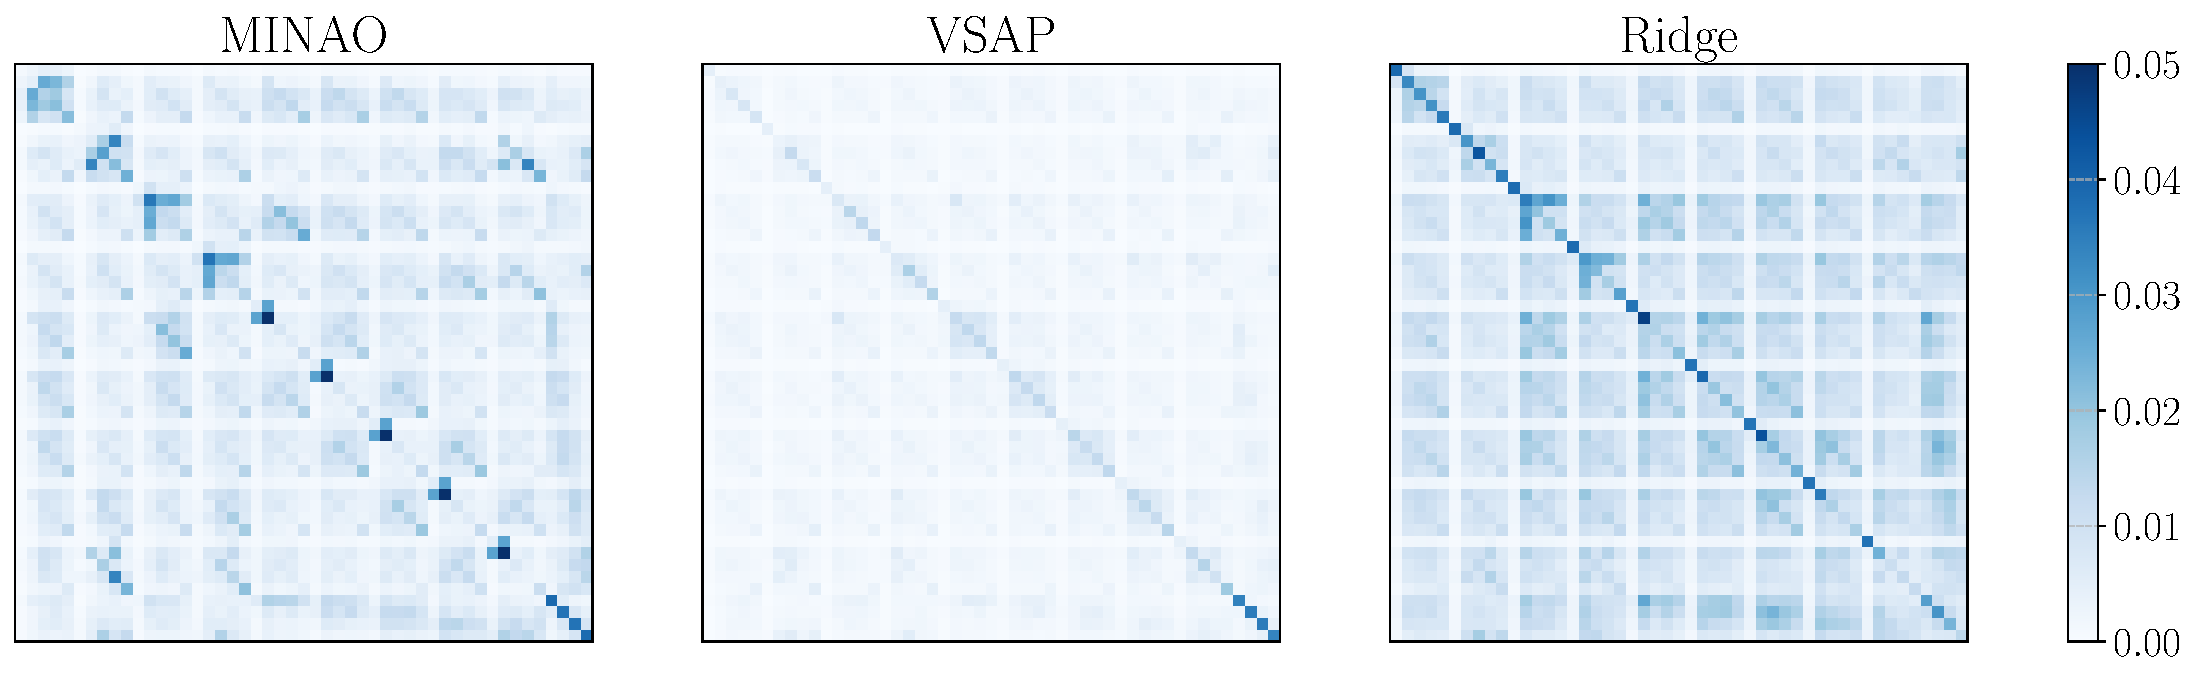
\includegraphics[width=\textwidth]{../fig/c5h4n2o2/density_error_comparison.pdf}
    \caption[Normalized difference of density guesses]{Normalized mean absolute difference of $\alpha$-electron density guesses to their converged density for \texttt{minao} \& \texttt{vsap} guess and the Ridge regression model evaluated on the testset: 102 (20\%) test samples from the \ch{C5H4N2O2} subset from QM9 \parencite{ref:article1_qm9}.}
    \label{fig:density_error_comparison}
\end{figure}
All three guessing schemes have spots on the main diagonal of the density matrix where they are likely to differ from the reference solution. Interestingly, a Mulliken population analysis (see \TODO{Background}) \parencite{ref:Mulliken_population_analysis} yields a mean value of $31.766$ the test set prediction for \texttt{minao} while \texttt{vsap} yield the expected $32$ (only $\alpha$-electrons). A small error in the initial guess doesn't slow down convergence, since the self-consistent cycle corrects it right away. Comparing \texttt{minao} and \texttt{vsap} with our Ridge Model the later fares worse on the main diagonal, especially for p-Orbitals. While \texttt{minao} exhibits more pronounced off-diagonal noise in comparision with \texttt{vsap}, this does not seem to affect convergence speed. At least for this small basisset it seems that errors in the off-diagonal do not hinder fast convergence.\\
% From that we might conclude that a good guess should be close to the reference density especially on the main diagonal, but not necessarily in the off-diagonal elements. We shall continue to investigate this in the next section.

\textbf{Kernel Ridge Regression}\\
Our baseline Ridge Regression (RR) model already introduced $L^2$-regularization handling collinearity which is doomed to happen in our dataset. However, it only models linear relationships between our input and output features. Kernel Ridge Regression (KRR) extends this by using kernel functions to generate a mapping from the input space via a higher dimensional feature space to the output space. This allows nonlinear relationships to be learned. \\
Using the same train/test split as before we train a KRR model with three different kernels: RBF, polynomial of degree 2 and polynomial of degree 3. 
Contrary to the mean-alpha heuristic given by the best performing target $\alpha$ value of the Ridge regression model, we use a global BayesSearch with 5-fold cross validation and 30 iterations\footnote{Search space: $\alpha \sim \operatorname{LogUniform}(10^{-8},10^{4})$, $\gamma \sim \operatorname{LogUniform}(10^{-6},10^{3})$, and $\mathrm{coef0} \sim \operatorname{Uniform}(0,1)$ for polynomial kernels; for the RBF kernel $\mathrm{coef0}$ is ignored} to obtain the results in \autoref{tab:kernel_ridge_metrics}.

\begin{table}[h]
    \centering
    \caption{Comparison of different guessing schemes for 102 (20\%) test samples from the \ch{C5H4N2O2} subset from QM9 \parencite{ref:article1_qm9}. The F-score is calculated using the Fock matrix prediction from the Kernel-Ridge regression model and the \texttt{minao} guess. The number of iterations until convergence is shown as well as the percentage samples not converging within 50 iterations and the inference time as a factor of the inference time of the minao guess.}
    \label{tab:kernel_ridge_metrics}
    \begin{tabular}{l
                    S[table-format=1.2(2)]
                    S[table-format=1.3(3)]
                    S[table-format=1.2(2)]
                    S[table-format=1.3(3)]}
        \toprule
        \textbf{Method} & \texttt{KRR-RBF} & \texttt{KRR-poly} & \texttt{1e} & \texttt{minao} \\
        \midrule
        F-score / 1         &  &  &  & 0.93 \pm 0.04 \\
        Iterations / 1      & 14 \pm 3 & 14 \pm 3 & 20 \pm 5 & 11.7 \pm 1.0 \\
        Not-Converged / \%  & 4 & 4 & 12 & 0\\
        Inference-speed / 1 &  &  &  & 1.0\\
        \bottomrule
    \end{tabular}
\end{table}

\TODO{Interpretation of results of KRR}

\textbf{Further trials \& other Basissize}\\
\TODO{Maybe add a bit more details about failed other trials on whole Fock-matrix}


\textbf{Predicting the Main Diagonal}
\TODO{Reference Cartus + GWH construction}
Previously we tried to learn a mapping from overlap to Fock matrix soley via machine learning means. We have established that the quality for these guesses even on the minimal STO-3G basis is not on par with the established guessing schemes.\\
Predicting the main diagonal for a given system is an easier target given the fact that the model predicts $N$ features from the $N^2$ input features. One established way of constructing the off diagonal elements is the generalized Wolfsberg-Helmholtz (GWH) construction \parencite{ref:gwh_wolfsberg1952spectra} (see \TODO{Background - guessing schemes}).

\textbf{Simple Multi Perceptron Regressor}\\


--- 
\begin{table}[h]
    \centering
    \caption{\TODO{\dots} Comparison of different guessing schemes for 102 (20\%) test samples from the \ch{C5H4N2O2} subset from QM9 \parencite{ref:article1_qm9}. The F-score is calculated using the Fock matrix prediction from the Ridge regression model and various guessing schemes implemented in \textsc{PySCF}. The number of iterations until convergence is shown as well as the percentage samples not converging within 50 iterations and the inference time as a factor of the inference time of the minao guess.}
    \label{tab:NN_basic_metrics}
    \resizebox{\textwidth}{!}{
    \begin{tabular}{l
                    S[table-format=1.2(2)]
                    S[table-format=1.3(3)]
                    S[table-format=1.2(2)]
                    S[table-format=1.3(3)]
                    S[table-format=1.3(3)]
                    S[table-format=1.3(3)]}
        \toprule
        \textbf{Method} & \texttt{NN-GWH-model} & \texttt{minao} & \texttt{1e} & \texttt{atom} & \texttt{huckel} & \texttt{vsap} \\
        \midrule
        F-score / 1 &  &  &  &  &  &  \\
        Iterations / 1 & 15 \pm 4 & 11.7 \pm 1.0 & 23 \pm 4 & 11.4 \pm 0.8 & 22 \pm 6 & 12.8 \pm 1.1 \\
        Not-Converged / \% & 4 & 0 &  32 & 0 & 28 & 0\\
        Inference-speed / 1 & 1.2 \pm 1.2 & 1.0 &  0.18 \pm 0.15 & 1.7 \pm 1.4 & 2.0 \pm 1.0 & 8 \pm 5 \\
        \bottomrule
    \end{tabular}
    }
\end{table}
---


Ideas: 
\begin{itemize}
    \item Maybe use spectral loss (eigenvalues?!) -> first ad hoc implementation didn't really work better
    \item CNN -> both okish on whole data but worse than ridge (without cycles benchmark) 
    \item NN  -> both okish on whole data but worse than ridge (without cycles benchmark)
    \item Maybe two step network -> first guess fock then get rid of noise? (open...)
    \item GWH construction -> first guess diagonal then use GWH to construct off-diagonal works ok for small set - worse for 6-32g(2d,f)
    \item Block guessing -> homo/hetero block guessing 
\end{itemize}


\section{Building guesses block-by-block}
\label{sec:blockwise_guessing}
\TODO{Guess main diagonal and then construct or guess off-diagonal elements.}

\TODO{Apply to larger basis sets.}